In order to test and evaluate the changes in BSE, a testing strategy consisting of a base line results from the original BSE. The new results when changes are made to the market will then be compared to these baseline results when ran with the same configuration of agents. These results illustrate the integrity of the market structure as well as the effects on the trading agents as their environment changes. 

\section{Base Line Results} 
Base Line results act as a standard which to be expected from the agents by running in a homogeneous market. These results are the indicator, apart from the unit and integration testing, that ensures the market is stabilized and performs as expected. The following graphs will illustrate the transaction prices in each homogeneous market. The following results are from running in the original BSE with equilibrium price of 70 in a homogeneous market with 7 agents on each side of the book. The period length (300), which is equivalent to 4200 McG time period and it is enough to illustrate how a market with ZIP agents transaction price converges to the equilibrium. 

\subsection{Kaplan's Sniper}
The Kaplan's Sniper is one of the agents implemented in the original version of ZIP. The sniper waits until near the end of the period, then submits or "snipe" its order. This is consistent with Figure 4.1 where the transaction only occurs near the end of the time period or when $t = 287$. 

\begin{figure}[!htbp]
\includegraphics[ height=8cm]{Dissertation/images/base_line/Sniper.png}
\caption{Sniper homogeneous transaction diagram with 70 price equilibrium} 
\end{figure} 
\FloatBarrier

\subsection{ZI-C}
ZI-C or Zero-Intelligence Constrained is another agent implemented in the original BSE. An expected behaviour of a market consisting of only ZI-C agents is a non-convergence transaction price. This is consistent with the Figure 4.2 below where at the end of the transaction period, the price does not converge to the equilibrium but instead exhibit a volatile price changes over the time period. 
\begin{figure}[h]
\caption{ZI-C homogeneous transaction diagram with 70 price equilibrium} 
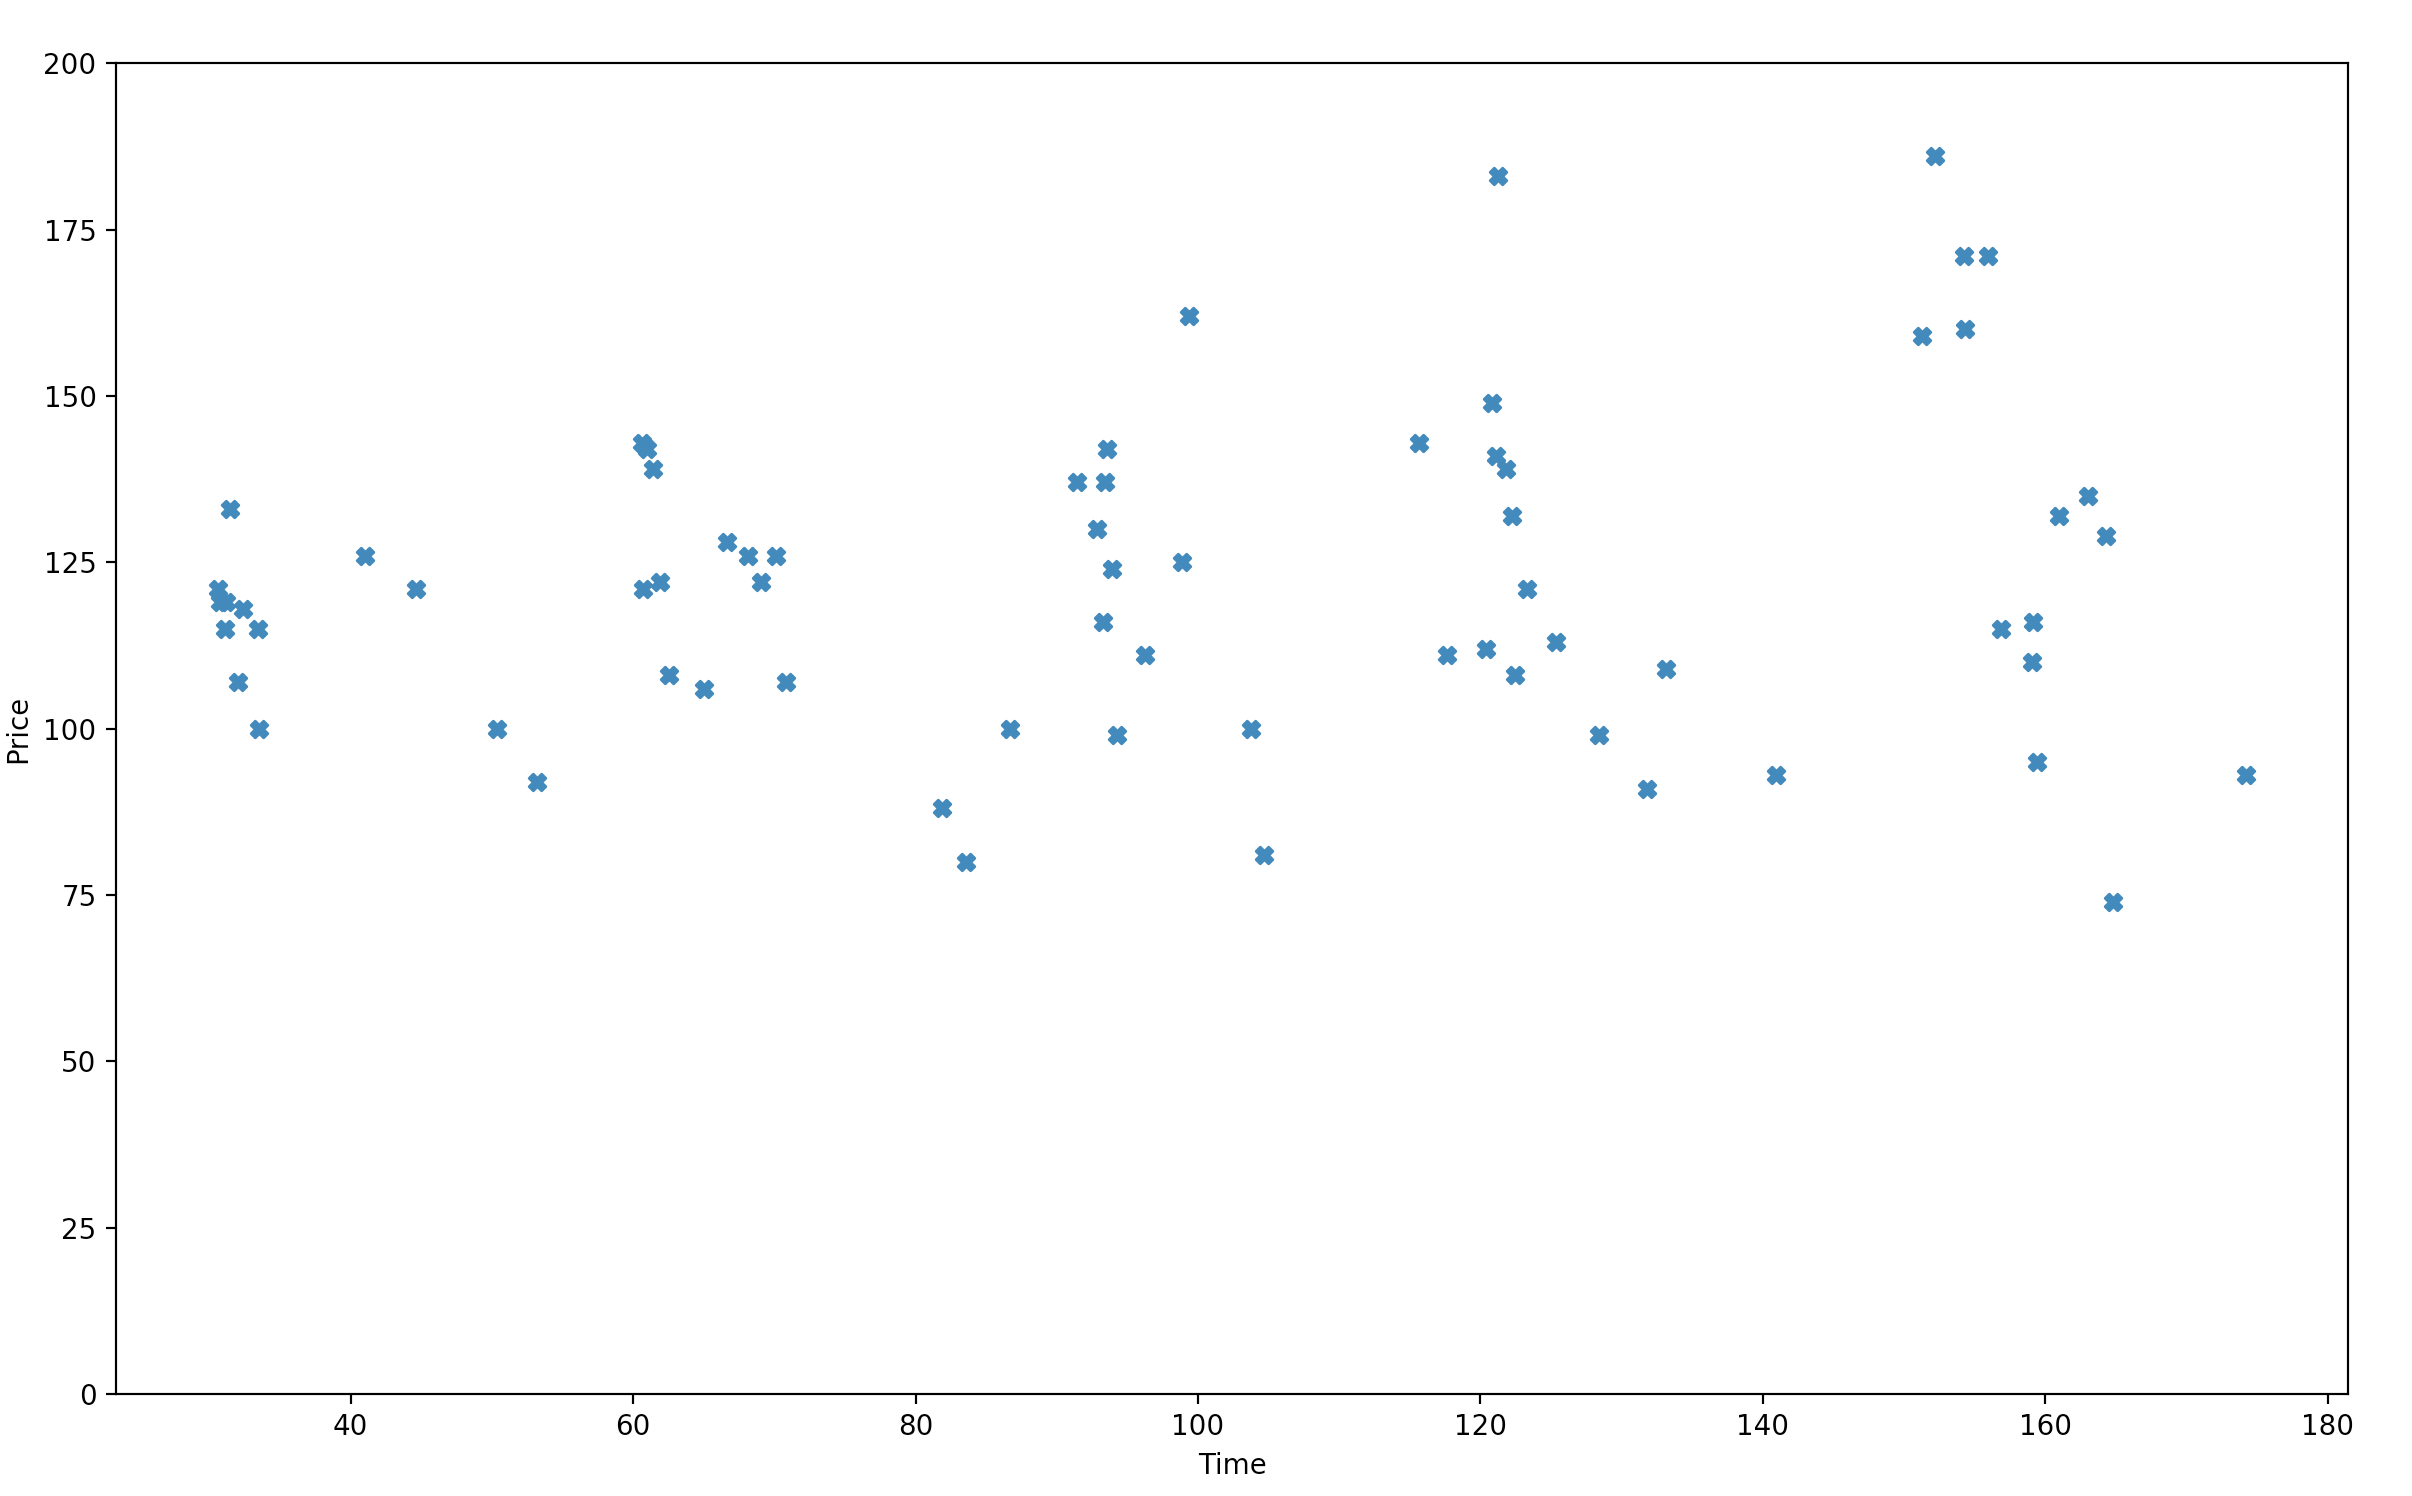
\includegraphics[ height=8cm]{Dissertation/images/base_line/ZIC.png}
\end{figure} 
\FloatBarrier

\subsection{ZI-P}
ZI-P or Zero-Intelligence Plus is the agent that, in a homogeneous market, does produce the transaction price which converges to the equilibrium. A market of ZI-P agents is a good indicator to test the market structure and functions. In the Figure 4.3 below, the transaction price first fluctuates early in the transaction period but then converges towards 70 in the end of the session.  
\begin{figure}[h]
\caption{ZI-P homogeneous transaction diagram with 70 price equilibrium} 
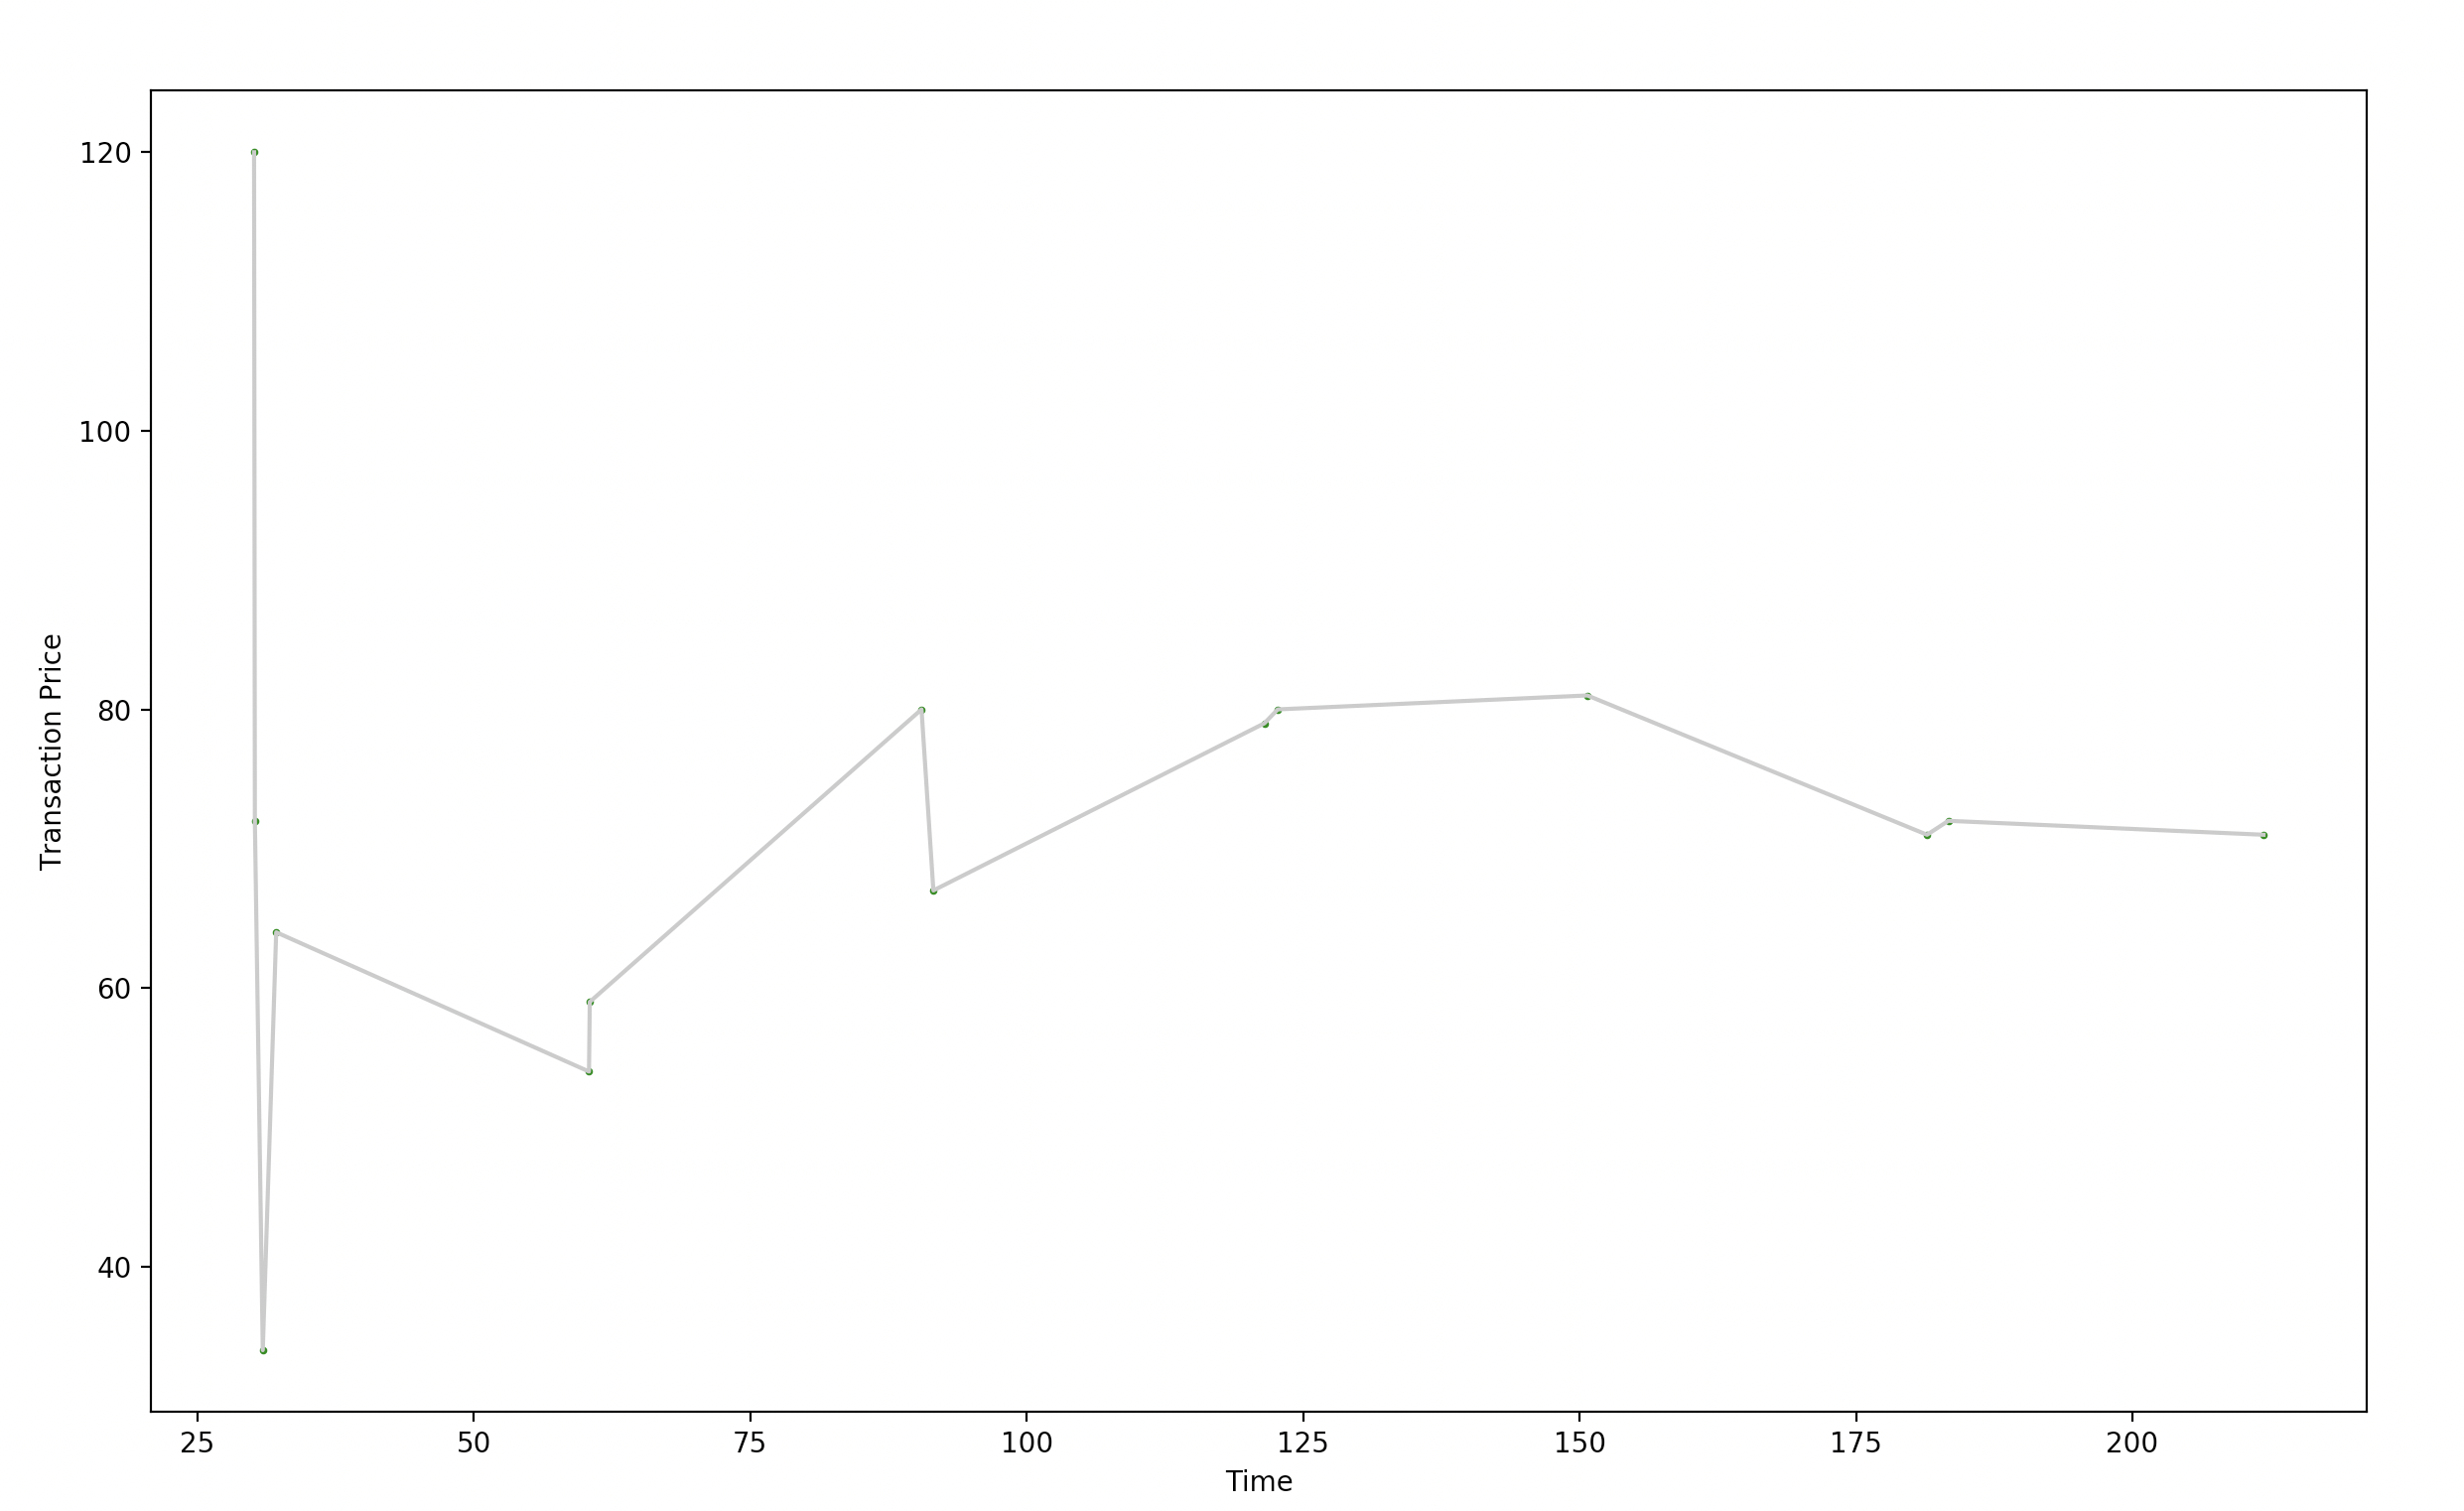
\includegraphics[ height=8cm]{Dissertation/images/base_line/ZIP.png}
\end{figure} 
\FloatBarrier

\section{Results after implementing complex order types} 
These results are from tests ran with the same configuration as the Base Line tests. These tests are ran after the LOB has been re-configured to be able to accept more than one type of order (Market Order as well as Limit Order) in addition to more than one quantity. The tests are ran with the same time step as the original BSE. 

\subsection{Kaplan's Sniper}
As expected, the Sniper only submits orders near the end of the session, which makes the first transactions only appear after $t = 245$.  
\begin{figure}[h]
\caption{Test 1 : Sniper homogeneous transaction diagram with 70 price equilibrium} 
\includegraphics[ height=8cm]{Dissertation/images/change1/Sniper.png}
\end{figure} 
\FloatBarrier

\subsection{ZI-C}
ZIC's behaviour in the new LOB is still similar to the one ran in the original BSE. The transaction price does not converge in any period of the session. 
\begin{figure}[h]
\caption{Test 1: ZI-C homogeneous transaction diagram with 70 price equilibrium} 
\includegraphics[ height=8cm]{Dissertation/images/change1/zic.png}
\end{figure} 
\FloatBarrier

\subsection{ZI-P}
ZIP illustrates a convergence to the 70 equilibrium as expected. 

\begin{figure}[h]
\caption{Test 1: ZI-P homogeneous transaction diagram with 70 price equilibrium} 
\includegraphics[ height=8cm]{Dissertation/images/change1/zip.png}
\end{figure} 
\FloatBarrier

\section{Results after implementing McG time step} 
This section illustrate the results with same test configurations on the BSE with McG time step. The McG time step is similar to the BSE except that it does not divide the individual time-step by the number of buyers and sellers then select them randomly. The McG time step loops through every trader in each time-step, allowing the trader to act in all the time steps. The time period selected is 4200 which is equivalent to the 300 time step in original BSE time-step. In addition, the interval is changed to be 10\% of the time-step for the customer order (price assignments) which is 420 in the McG and 30 in the original BSE. The results of the tests are illustrated below. 

\subsection{Kaplan's Sniper}
As expected, the Sniper only submits orders near the end of the session, which makes the first transactions only appear after $t = 3400$.  
\begin{figure}[h]
\caption{Test 2 : Sniper homogeneous transaction diagram with 70 price equilibrium} 
\includegraphics[ height=8cm]{Dissertation/images/change2/Sniper.png}
\end{figure} 
\FloatBarrier

\subsection{ZI-C}
ZIC's behaviour in the new LOB is still similar to the one ran in the original BSE. The transaction price does not converge in any period of the session. 
\begin{figure}[h]
\caption{Test 2: ZI-C homogeneous transaction diagram with 70 price equilibrium} 
\includegraphics[ height=8cm]{Dissertation/images/change2/zic.png}
\end{figure} 
\FloatBarrier

\subsection{ZI-P}
ZIP illustrates a convergence to the 70 equilibrium as expected. 

\begin{figure}[h]
\caption{Test 2: ZI-P homogeneous transaction diagram with 70 price equilibrium} 
\includegraphics[ height=8cm]{Dissertation/images/change2/zip.png}
\end{figure} 
\FloatBarrier
